\documentclass[12pt, a4paper]{report}
\usepackage[T1]{fontenc}
\usepackage{inputenc}
\usepackage{pdfpages}
\usepackage[toc]{glossaries}
\usepackage{booktabs}
\usepackage{float}
\usepackage{hyperref}
\usepackage{mathtools}
\hypersetup{
    colorlinks,
    citecolor=black,
    filecolor=black,
    linkcolor=black,
    urlcolor=black
}

\makeglossaries
\newglossaryentry{mmal}
{
  name=mmal,
  description={is a programmable machine that receives input,
               stores and manipulates data, and provides
               output in a useful format}
}

\usepackage{tabularx}
	\newcolumntype{L}{>{\raggedright\arraybackslash}X}


\begin{document}

\begin{titlepage}

\newcommand{\HRule}{\rule{\linewidth}{0.5mm}} % Defines a new command for the horizontal lines, change thickness here

\center % Center everything on the page

\textsc{\LARGE ZHAW School of Engineering}\\[1.5cm] % Name of your university/college
\textsc{\Large Projektarbeit}\\[0.5cm] % Major heading such as course name
\textsc{\large IT}\\[0.5cm] % Minor heading such as course title

\HRule \\[0.4cm]
{ \huge \bfseries Title}\\[0.4cm] % Title of your document
\HRule \\[1.5cm]


\begin{minipage}{0.4\textwidth}
\begin{flushleft} \large
\emph{Authors:}\\
Linda Helen \textsc{Boedi}  Valentin \textsc{Bossi} % Your name
\end{flushleft}
\end{minipage}
~
\begin{minipage}{0.4\textwidth}
\begin{flushright} \large
\emph{Supervisor:} \\
 \textsc{Gelke} % Supervisor's Name
\end{flushright}
\end{minipage}\\[2cm]


{\large \today}\\[2cm] 

%
\includegraphics{logo.png}\\[1cm] 

\vfill 

\end{titlepage}

\chapter{Acknowledgement}

\chapter{Affidavit}

\setcounter{secnumdepth}{5} 
\setcounter{tocdepth}{5} 
\tableofcontents

\chapter{Conceptual formulation}

\chapter{Motivation}

\chapter{Fundamentals}
\section {Competitor Analysis}
\subsection{Optical versus acoustical measurement}
To measure the frequency of the balance wheel of a mechanic clock there exist mainly two methods on the market, acoustical and optical measurement. The common used method is by analyzing the noises of the balance wheel. More expensive devices use both acoustical and optical feedback.

\begin{table}
 \centering
\begin{tabularx}{\linewidth}{ |c||L|L|  }
 \hline
 \multicolumn{3}{|c|}{\textbf{Comparison acoustical and optical measurement}} \\
 \hline
 & \textbf{acoustical}  & \textbf{optical} \\\hline
  since   &  around 19th century (2)  & end of 20th century (2)\\ \hline
 accuracy &   0.1 s/d & 0.1 s/d\\  \hline
 advantages & most experience (exists for about 200 years)& measurement can be done anywhere\\  \hline
 disadvantages & background noises need to be filtered out& \\
 \hline
\end{tabularx}
    \end{table}

\subsubsection{Acoustical measurement}
The first used method to get the frequency measurement of the balance wheel was by using a vibrograph was used. For every "tick" of the clock a line was drawn onto a ongoing strip of paper. Out of the distance between of these lines the frequency was calculated. (1) But as this method isn't the most accurate other techniques are used nowadays.  
Modern watch timing machines use an oscillating quartz crystal as comparison for the frequency of the balance wheel (1). The noises of the balance wheel are recorded and amplified with a microphone whereat unwanted background noises need to be filtered out. 

\subsubsection{Optical measurement}
About hundred years later, optical watch timing machines joined the acoustical ones. There are barely devices on the market, which use only optical measurement, but several companies started to combine their acoustical with optical metering. One way to scale the frequency of the balance wheel optically is by using a laser. The beam will be periodically interrupted by the balance wheel and thus the frequency can be calculated (3). In this paper the frequency should be quantified optically by using image processing. There is hardly to none company out there, which uses the last technique for measuring the frequency.

\subsection{Companies}
\subsubsection{Witschi - WisioScope S}
WisioScope S tests mechanical watches acoustically and optically. The measurement is done parallel and in this way is more accurate as both signals are used for the calculation of the frequency.
The optical metering is done using a laser and lighting, a camera helps to adjust the watch properly. The costs of their product are: CHF 10450.-

\bigskip

\begin{tabularx}{\textwidth}{>{\bfseries}lX}
Measurement gear deviation & \\\toprule
scope & +/- 999.9 s/d \\\midrule
resolution & 0.1 s/d\\\bottomrule
\end{tabularx}

\subsubsection{Lepsi - WatchScope/WatchAnalyzer}
The WatchScope and WatchAnalyzer by Lepsi are mostly for enthusiasts and not really for the manufacturing. Both devices only work with acoustical input. All data can be accessed with the smartphone. The prices of their product are CHF 369.-, resp. CHF 929.-

\subsubsection{Greiner Vibrograf - Compact 900}
The Compact 900 measures only the beat noises of the balance wheel. The price is CHF 4070.-

\section{Reference measurement and test watch}
At first some general information to the test watch, which was used.

The test watch is a watch of the caliber ETA C01.211 it is a chronograph, with a diameter of 31 centimeters. It has a beat rate of 21600 beats per hour and therefore a frequency of 3 Hz. Additionally the watch has a power reserve of 43 hours. (5)

In order to obtain an exact reference value of the frequency of the balance wheel of the test watch, an acoustic measurement was carried out with a professional measuring device, the Greiner Vibrograf - Compact 900, and the rate deviation was determined. 

In order to calculate the frequency from the gear deviation of the balance wheel, first some transformations had to be carried out. 

Since the rate deviation has been calculated in seconds per day and the number of strokes per hour, i. e. the number of audible impulses (beats) of a two-armed armature of a mechanical watch per hour, is known, these two quantities must first be brought to a unit. The relationship between the beat number (n*) and frequency (f) is as follows: 

\begin{displaymath}
n* = 2f*3600
 \end{displaymath}
 and therefore:
 \begin{displaymath}
  f = \frac{n*}{7200}
 \end{displaymath}

\chapter {Experimental approaches}

\section {Evaluation of possible technologies}
\subsection{Frame analysis versus given GPU motion vectors}
One approach is to compare each image with the subsequent image and to mark the displacements with motion vectors. This would mean a considerable computational effort.
Such motion vectors are already made by the GPU, in order to compress videos in the H.264 codec.

\subsection{Frame analysis via OpenCV}
With the library OpenCV it is possible to determine the optical flow of an image sequence. 

The optical flow represents the vector field of the velocities of the points of an image sequence. It is a useful representation of motion information in image processing. The local optical flow is an estimate of patterns in an image in the vicinity of a viewed pixel. 

One possibility would be to follow the course of a velocity vector and thereby calculate a period of the frequency of the balance wheel. The calculation of the flow at selected points is also called feature point tracking. Another approach would be to calculate the frequency based on the velocity obtained from the optical flow, since it is more or less a circular movement. 

One difficulty with this procedure is that one has to commit to certain pixels that one examines. This can cause problems if the clock is placed differently, because wrong points (worst-case scenario: points in which movement never takes place) can cause problems for the calculation.  

The OpenCV library uses the Lucas-Kanade method to calculate the optical flow. The Lucas-Kanade method also assumes that the flow in the local environment of the pixel for which the flow is intended is the same. So more or less a whole set of pixels is considered. The flow can thus be determined by calculating the derivatives (= gradients). 

One characteristic of this method is that it does not provide a dense flow, i. e. the flow information disappears quickly with the distance from the edges of the image. The advantage of the method is its relative robustness against noise and smaller defects in the image.

\subsection{Motion vectors from high level library picamera}
The picamera library is capable of storing all motion vector estimations of the h.264 encoder in an object. This object with all motion vectors for all frames can be later accessed and used. The motion data is at the level of macro-blocks where the values are 4-bytes long and consist of a signed 1-byte x vector, a signed 1-byte y vector and an unsigned 2-byte SAD (Sum of Absolute Differences) value. All motion data values can be easily accessed frame by frame. (2) 

The sum of absolute differences is a positive number resulting from the formation of the difference between two digital images. It serves as a measure of the difference between two images.

The SAD is obtained by subtracting the color values of the images pixel by pixel from each other and adding them up by amount. (3)

The advantage of the Picamera library is that compared to the possibilities of the OpenCV library, the information about the motion vectors is available faster, since this library already has an internal object (motiondata), which stores all necessary information as well as the SAD value. 

\section{Animation of motion vectors}
After deciding which library to use, some experimental sessions took place to get a better understanding of the so called motion data values or motion vectors. 
With the picamera library it is easy to access these motion data values so the hard part wasn't to get the values but to understand how they are constructed. 
The motion data object consists of multiple values; a signed 1-byte x vector, a signed 1-byte y vector and and unsigned 2-byte SAD value for each macro-block of a frame.

In a first step all SAD values were animated with colors to get a better understanding of how good the information they keep is and how as well as if they can be used to calculate the frequency of the movement of the balance wheel.

\bigskip

\noindent
\begin{center}
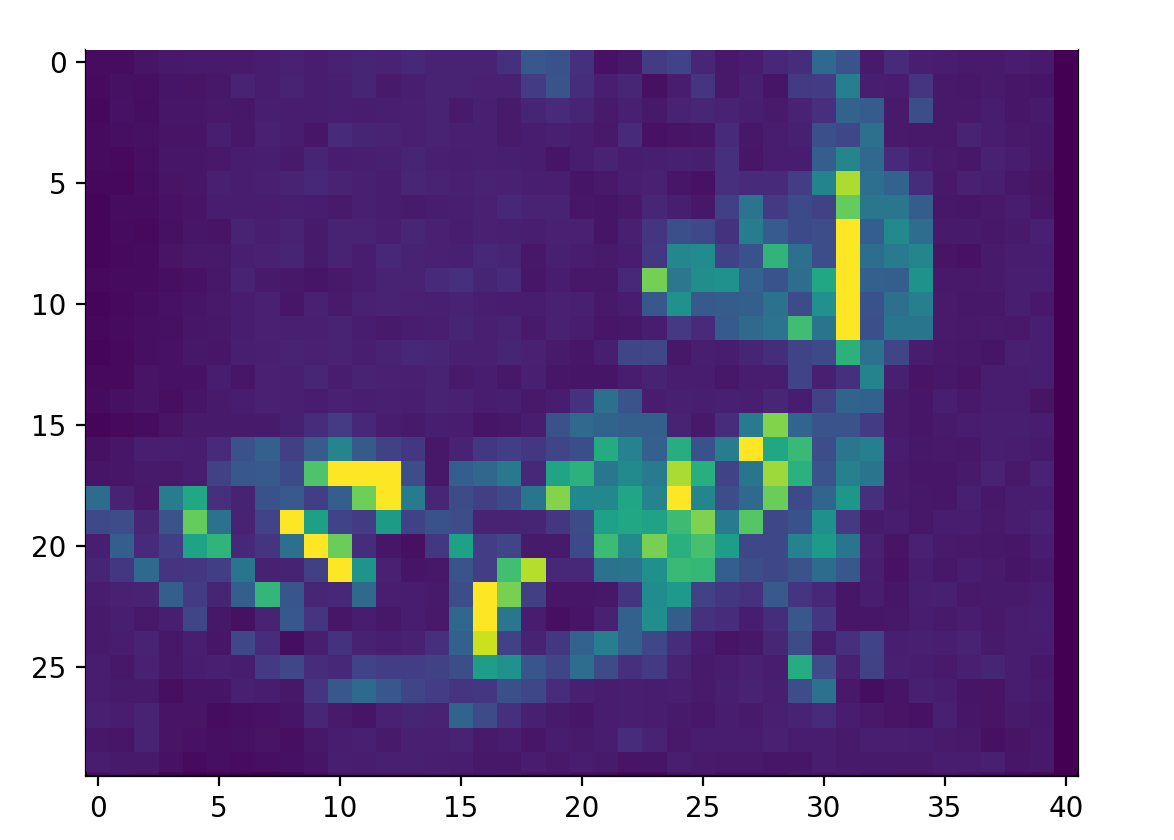
\includegraphics[scale=0.6]{Images/animation_sad.png}

{\bf Illustration 1:}  Animation of the SAD values, the lighter the color the higher the value of the SAD
\end{center}

\bigskip
 
Further the x and y vector were analyzed and also animated. But as those vectors itself are hard to use and give incomplete information (WHY?), the hypotenuses were calculated with Pythagoras' theorem and displayed similar to the SAD values. The hypotenuses give information about the amount as well as the direction of the motion.
 
 \bigskip

\noindent
\begin{center}
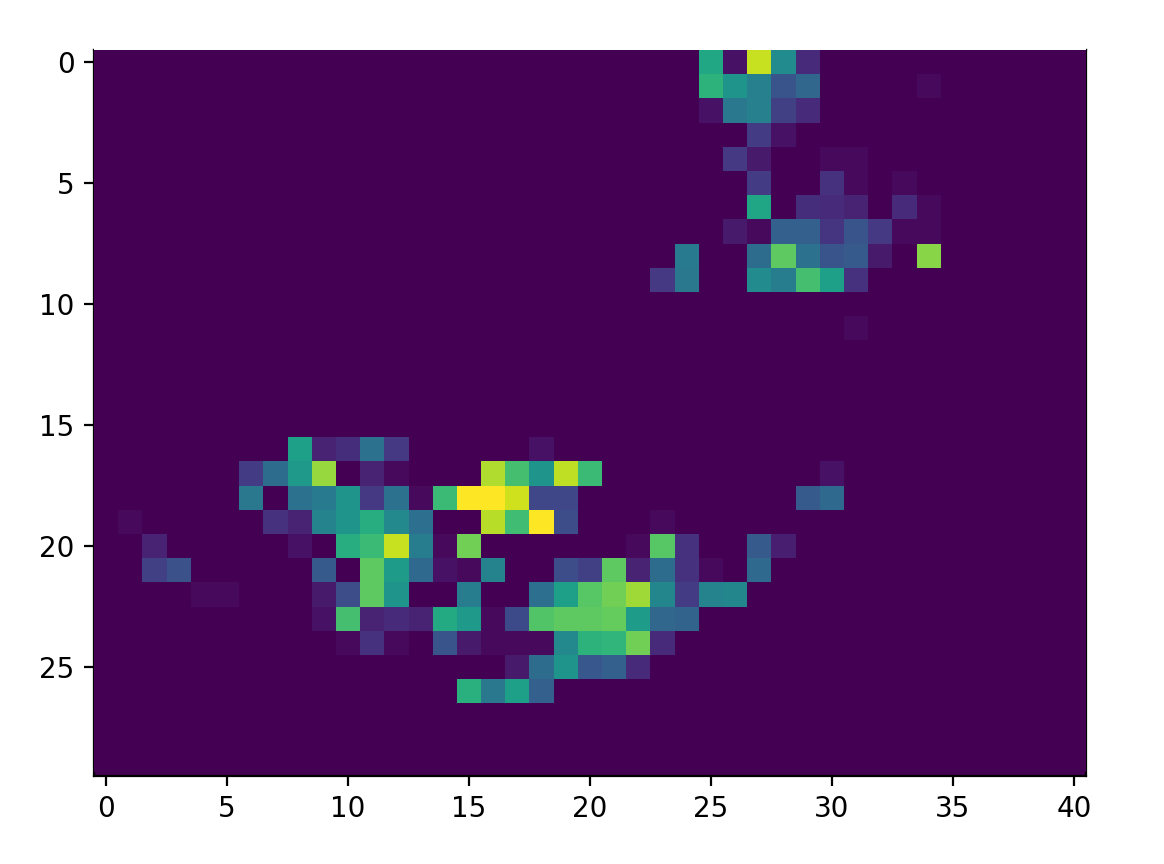
\includegraphics[scale=0.6]{Images/animation_hypotenuse.png}

{\bf Illustration 2:}  Animation of the hypotenuses, the lighter the color the higher the value of the hypotenuse
\end{center}

\bigskip

Another experimental approach was displaying the motion vectors as arrows directly in the video. This approach was helpful to get a better understanding under which conditions the best result of the motion vectors is reached.
\pagebreak

\subsection{Motion vectors visualized in a frame}
Codecvisa was used to display the motion vectors of a frame.
The result is shown in Figure 3.
\bigskip
\noindent
\begin{center}
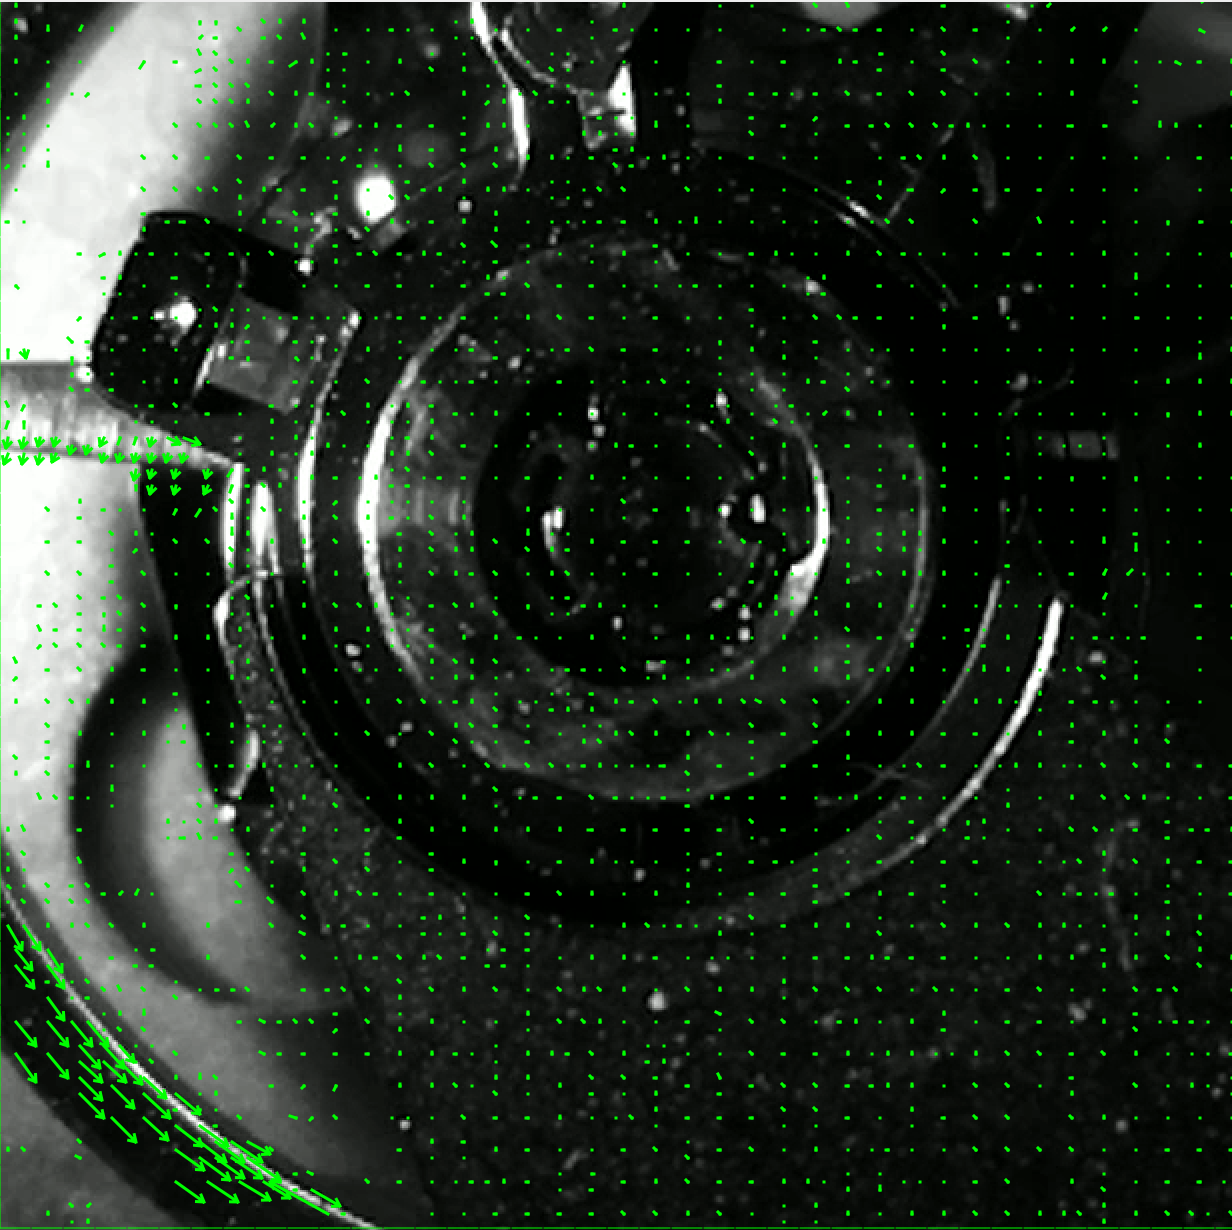
\includegraphics[scale=0.4]{Images/motion_vectors.png}

{\bf Illustration 3:}  Motion vectors drawn in one frame
\end{center}
\bigskip

Another approach used Excel was to determine whether a motion vector from one frame is the predecessor of the motion vector in the next frame.
The hope was that a moving pixel could be followed and therefore the location of the pixel would always have been known.
The result was sobering because one frame and motion vector cannot be associated with another frame and motion vector.
This experiment looked at the idea of the optical flux with the movement vectors of the MMAL (Multi-Media Abstraction Layer).

\noindent
\begin{center}
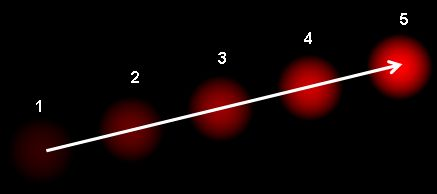
\includegraphics[scale=0.55]{Images/optical_flow_basic1.jpg}

{\bf Illustration 4:}  It shows a ball moving in 5 consecutive frames. The arrow shows its displacement vector.
\end{center}

\bigskip

\section{Picamera library}

\section{Crude calculation of frequency}
With the help of the motion vectors and the corresponding time stamps per frame, a rough calculation of the frequency can be made.
All x, y or SAD values contained in the image are summed up. If the sum of all values is small, it is very likely that the balance will not move so that it is at a standstill.
For small values, the time stamp is registered and the difference to the next standstill is calculated.
Since the balance wheel triggers half a oscillation, it has moved from one stop to the next half point. 
 
\chapter{Calculation of the frequency}

\section{Implementation of the algorithm}

In a next step, the results of the rough calculation from the Excel sheet were transferred into a Python program. 

The greatest difficulty proved to be the detection of the minimia, which characterize the standstill of the balance wheel. These were relatively easy visible to the unaided eye, but in an automatic calculation, appropriate conditions had to be set in order to take into account the correct values and correct the inaccuracies caused by the noise. The setting of an upper limit for the minima proved to be a suitable condition. All minima below this limit are therefore taken into account. 

Furthermore, the calculation of the frequency in the Python program has been further simplified by not calculating each period individually, but by selecting the first and the last minimum over the whole period of time, in which it was recorded. This time span is then calculated by half of the number of minima minus 1. Half, because every half of the period the balance wheel stops and minus 1, because otherwise a half-period would be taken into account too much. This approach reduces the number of rounding errors, resulting in higher accuracy. After this calculation, the period duration T is now available, from which the frequency f can be calculated quite simply: 

 \begin{displaymath}
  f = \frac{1}{T}
 \end{displaymath}

\chapter{Results}

\section{Measurements}
This measurements were taken in different positions of the watch with different length
of recordings. Each position were recorded in 10, 20, 40 and 80 minutes.

Figure 5 and Table 3 shows the deviation per day based on the following calculation:
Taken the first timestamp (t1) of a stillstand and taken the last timestamp (t2) of a stillstand, the counted
number of stillstands (s1), number of strokes per hour (s2) (21600):
\bigskip

\(t2-t1 = \triangle t\)

\(\triangle t / s = f*2\)

\((f*2*s2)-3600=deviation per hour\)

\begin{center}
    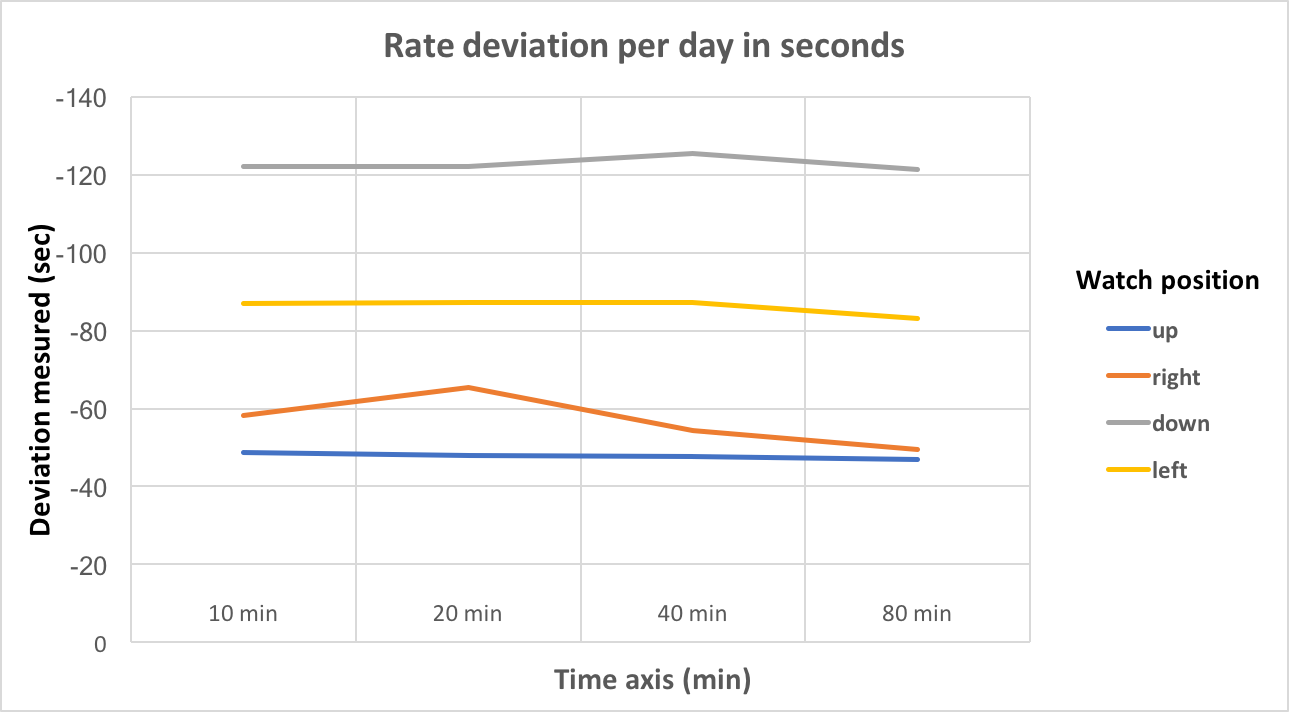
\includegraphics[scale=0.3]{Images/variations_per_day.png}
    
    {\bf Illustration 5:} Variation of different time and position recordings
    \end{center}
\begin{table}[H]
    \begin{tabular}{|l|l|l|l|l|l|}
    \hline
    Positions & Greiner Compact 900 & 10 min & 20 min & 40 min & 80 min \\ \hline
    up        & -13                 & -48.7     & -48.0     & -47.6      & -47.0      \\ \hline
    right     & -30                 & -58.3      & -65.5    & -54.4      & -49.4      \\ \hline
    down      & -20                 & -122.2    & -122.2     & -125.4    & -121.4      \\ \hline
    left      & -14                 & -87.0	   & -87.1	  & -87.1	  & -83.1      \\ \hline
    \end{tabular}
\end{table}
\begin{center}    
{\bf Table 3: variations per day in seconds} 
\end{center}

\bigskip

\begin{center}
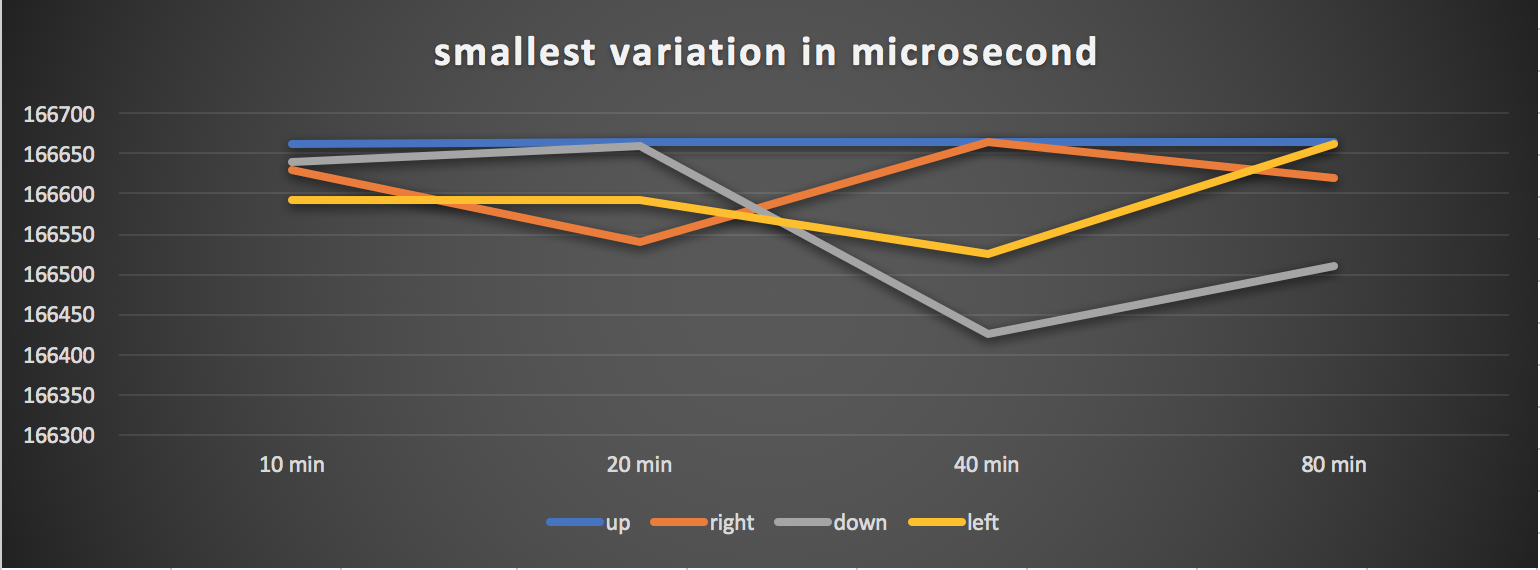
\includegraphics[scale=0.3]{Images/smallest_variation.png}

{\bf Illustration 6: Variation of different time and position recordings}
\end{center}
\begin{table}[H]
    \begin{tabular}{|l|l|l|l|l|l|}
    \hline
    Positions & Greiner Compact 900 & 10 min & 20 min & 40 min & 80 min \\ \hline
    up        & -13                 & -2.9     & -0.8     & -1.3      & -0.8      \\ \hline
    right     & -30                 & -19      & -65.6    & -0.8      & -24.7      \\ \hline
    down      & -20                 & -13.8    & -3.4     & -125.2    & -81.7      \\ \hline
    left      & -14                 & -39.2	   & -39.2	  & -72.9	  & -2.9      \\ \hline
    \end{tabular}
\end{table}
\begin{center}    
{\bf Table 4: variations per day in seconds based on smallest variation} 
\end{center}

\section{Evaluation}


\pagebreak

\chapter{Appendices}

\begin{thebibliography}{9}
\bigskip
\bibitem[Uhrenwiki]{Uhrenwiki} 
(1) https://www.uhren-wiki.net/index.php?title=Zeitwaage
\bibitem[ncsli]{ncsli} https://www.ncsli.org/c/f/p11/286.314.pdf
\bibitem[chronoscop]{chronoscop} http://www.chronoskop.com/index.php/chronoskop-zeitwaagen-von-prelislisit-timegraphers/
\bibitem[Picamera]
(2) picamera readthedocs
\bibitem[SAD]
(3) Wikipedia: Sum of absolute differences
\bibitem[Schlagzahl]
(4) Wikipedia: Schlagzahl
\bibitem[Caliber Test watch]
(5) http://watchbase.com/eta/caliber/c01-211
\end{thebibliography}

\pagebreak

\section {Illustration directory}
\bigskip

\begin{itemize}
\item Abbildung 1: Animation SAD values. Linda Boedi and Valentin Bossi
\item Abbildung 2: Animation hypotenueses. Linda Boedi and Valentin Bossi
\end{itemize}

\end{document}
